%%%%%%%%%%%%%%%%%%%%%%%%%%%%%%%%%%%%%%%%%%%%%%%%%%%%%%%%%%%%%%%%%%
\subsection{Random Forest (\acrshort{rf})}
\label{sec:rf}

\subsubsection{Puntuación de características}
\label{sec:rf1}

Se desarrolla una primera versión del clasificador basado en la técnica de \gls{rf}, \textit{RandomForestClassifier()}, para visualizar las características que más repercuten en el proceso de clasificación de errores. En este modelo por defecto, se construyen un total de 10 estimadores o árboles y se determina el criterio de medición de la impureza a partir de la entropía (ver Sección \ref{sec:mlrf}). Después, se aplican dos métodos diferentes para puntuar la importancia que toman las características en el clasificador anterior. 

\vspace{3mm}

\begin{lstlisting}[style=Python, caption={Clasificador RF por defecto}]
  classifier = RandomForestClassifier(n_estimators = 10, criterion = 'entropy', random_state = 0) 
  classifier.fit(X_train, y_train)
\end{lstlisting}
  
\vspace{3mm}

Por un lado, se estima la importancia de las características del conjunto, a partir del atributo \textit{feature\_importances\_}, proporcionado por el clasificador \gls{rf}. En este caso, el cálculo se realiza a partir de la media y de la desviación estándar de la disminución de la impureza que se produce dentro de cada árbol. Como se representa en la Figura \ref{fig:imp1}, se devuelve un array con los valores de importancia relativa asignados a las características y cuyo sumatorio es igual a 1. En este caso, se visualiza una gran incidencia de la distancia, seguida de los parámetros resultantes de \gls{den2ne}, \textit{total\_balance} y \textit{abs\_flux}, que hacen referencia a la carga que presenta el nodo \textit{gateway} tras el balance y al flujo total de recursos intercambiados en el proceso de distribución energética.

\vspace{3mm}

Sin embargo, con este método surgen cierto sesga hacia las características que presentan alta cardinalidad, o en otros términos, una gran cantidad de valores únicos. Esto se debe a que generan nodos de división con mayor profundidad en los árboles, puesto que existen más opciones de separación del conjunto de datos. Por lo tanto, este tipo de características pueden recibir una puntuación más inflada. Teniendo esto en cuenta, se decide cuantificar la importancia también por el método de permutación (\textit{permutation\_importance}). Como se puede ver en la Figura \ref{fig:imp2}, en este caso, los parámetros resultantes de \gls{den2ne}, \textit{total\_balance} y \textit{abs\_flux}, siguen presentando puntuaciones altas, pero ahora también, las longitudes de las etiquetas de los nodos y la capacidad del enlace. \cite{importance}

\begin{figure}[H]
  \centering
  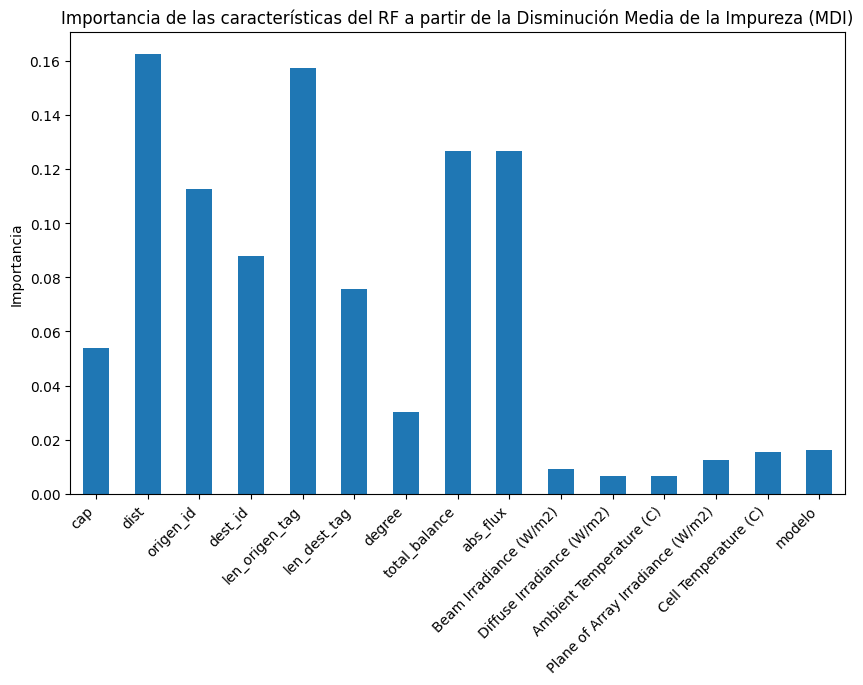
\includegraphics[width=1\textwidth]{img/desarrollo/rf/importance1.png}
  \caption{Puntuación de características del \acrshort{rf} mediante el atributo \textit{feature\_importances\_}}
  \label{fig:imp1}
\end{figure}

\begin{figure}[H]
  \centering
  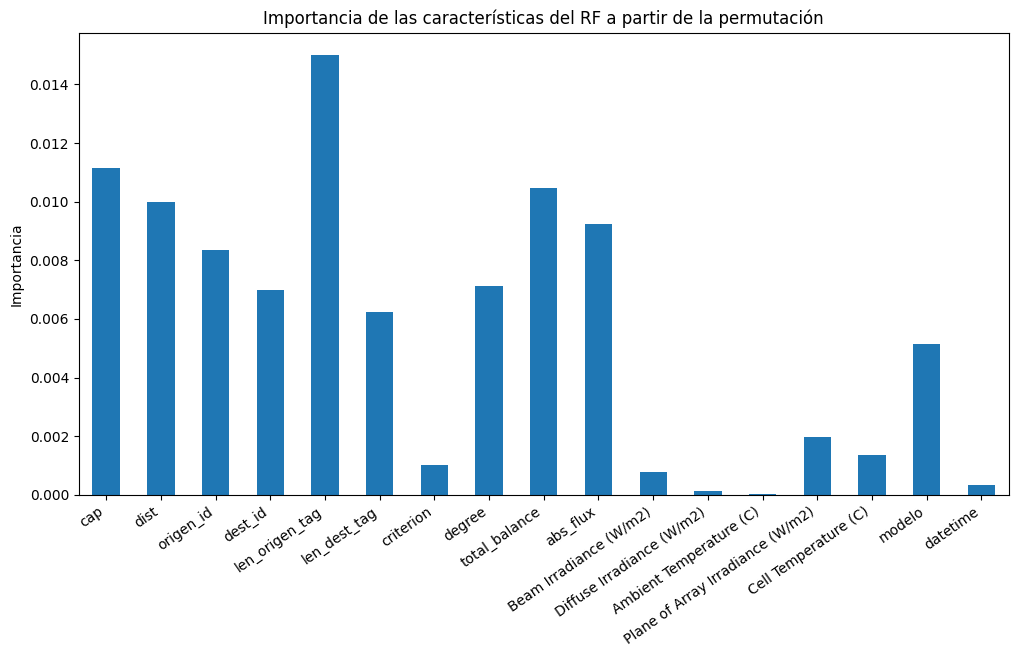
\includegraphics[width=1\textwidth]{img/desarrollo/rf/importance2.png}
  \caption{Puntuación de características del \acrshort{rf} mediante el método \textit{permutation\_importance}}
  \label{fig:imp2}
\end{figure}

En este segundo método los valores de las características se permutan una a una aleatoriamente y se evalúa en cada iteración los resultados del clasificador. Por tanto, cuando la variación de valores de una característica decrementa de forma considerable la precisión del modelo, puntúa una mayor importancia. Esta técnica es útil porque proporciona una evaluación imparcial de la importancia de las características. 

\subsubsection{Optimización de hiperparámetros}

Los hiperparámetros de un modelo se tratan de los parámetros de configuración o argumentos que son incluidos en el constructor de la clase del estimador o clasificador. En el caso del \gls{rf}, como ya se había introducido en el diseño del modelo por defecto, se pone el foco en dos hiperparámetros principales: el número de estimadores o árboles y el criterio de medición de la impureza. Para encontrar los valores que construyen el modelo óptimo de \gls{rf}, es preciso emplear la técnica \textit{Grid Search} \cite{gridsearch} y, específicamente, la clase \textit{GridSearchCV()} \cite{gridsearch2}. Esta realiza una búsqueda exhaustiva a partir de la definición de una cuadrícula de hiperparámetros para el estimador y extrae la combinación de valores que aporta una mayor precisión. Por ello, es necesario primero, definir en un diccionario una serie de valores para los dos hiperparámetros que se pretenden optimizar en el nuevo clasificador.

\vspace{3mm}

\begin{lstlisting}[style=Python, caption={Cuadrícula de parámetros}]
  param_grid = {
    'n_estimators': [10, 25, 50, 75, 100],
    'criterion': ['entropy', 'gini']
  }
\end{lstlisting}

\vspace{3mm}

Por consiguiente, se crea el objeto de la clase \textit{GridSearchCV()} y se determina el esquema de validación cruzada (\textit{cross validation}) de este mediante el parámetro \textit{cv}. En este caso, toma un valor de 5 y define el número de pliegues (\textit{folds}) que se van a utilizar para dividir el conjunto de datos y evaluar las combinaciones de los hiperparámetros. De la misma forma, se especifican el resto de parámetros, como la métrica para evaluar el rendimiento del modelo en cada iteración, que viene dada por la precisión global obtenida (\textit{accuracy}). 

\vspace{3mm}

Una vez creado el objeto, se ajusta al conjunto de datos de entrenamiento. Este proceso, a partir de los atributos \textit{best\_score\_} y \textit{best\_params\_}, aporta a la salida cuál es la mejor combinación de parámetros de todas las probadas y qué valor de precisión alcanza la misma. En este caso, se obtiene una precisión del 99,18\% con un clasificador basado en 100 estimadores y en el criterio de entropía. 

\vspace{3mm}

\begin{lstlisting}[style=Python, caption={Construcción del objeto \textit{GridSearchCV()}}]
  grid_search = GridSearchCV(estimator = classifier,
                            param_grid = param_grid,
                            scoring = 'accuracy',
                            cv = 5,
                            n_jobs = -1)

  grid_search.fit(X_train, y_train)
\end{lstlisting}

\vspace{3mm}

Sin embargo, para llevar a cabo un análisis en mayor profundidad de los resultados, se hace uso del atributo \textit{cv\_results\_}, que proporciona un diccionario con toda la información útil de la búsqueda. Principalmente, este análisis se centra en los valores de precisión obtenidos de todos los modelos y en los tiempos promedios que han sido necesarios para ajustar los mismos al conjunto de entrenamiento. Como se puede apreciar en la Tabla \ref{tab:rfgs}, se presentan variaciones muy pequeñas en los valores de precisión obtenida (\textit{mean\_test\_score})para las diferentes combinaciones de parámetros.

\vspace{3mm}

\begin{table}[H]
  \centering
  \begin{subtable}{0.45\linewidth}
    \centering
    \begin{tabular}{|>{\columncolor[HTML]{EFEFEF}}c |c|c|}
      \hline
      \textit{\begin{tabular}[c]{@{}c@{}}Criterio /\\ Nº estimadores\end{tabular}} & \cellcolor[HTML]{EFEFEF}\textit{Entropía} & \cellcolor[HTML]{EFEFEF}\textit{Gini} \\ \hline
      10 & 99,07 & 99,02 \\ \hline
      25 & 99,16 & 99,14 \\ \hline
      50 & 99,16 & 99,15 \\ \hline
      75 & 99,17 & 99,17 \\ \hline
      100 & 99,18 & 99,16 \\ \hline
    \end{tabular}
    \caption{Precisión (\%) (\textit{mean\_test\_score})}
    \label{tab:rfgs}
  \end{subtable}
  \hfill
  \begin{subtable}{0.45\linewidth}
    \centering
    \begin{tabular}{|>{\columncolor[HTML]{EFEFEF}}c |c|c|}
      \hline
      \textit{\begin{tabular}[c]{@{}c@{}}Criterio /\\ Nº Estimadores\end{tabular}} & \cellcolor[HTML]{EFEFEF}\textit{Entropía} & \cellcolor[HTML]{EFEFEF}\textit{Gini} \\ \hline
      10 & 147 & 146 \\ \hline
      25 & 373 & 382 \\ \hline
      50 & 747 & 761 \\ \hline
      75 & 1072 & 1002 \\ \hline
      100 & 1439 & 987 \\ \hline
    \end{tabular}
    \caption{Tiempo (s) (\textit{mean\_fit\_time})}
    \label{tab:rfgs2}
  \end{subtable}
  \caption{Resultados extraídos del atributo \textit{cv\_results\_} del \textit{Grid Search} en el \acrshort{rf}}
  \label{tab:rfgs_combined}
\end{table}

\vspace{3mm}

No obstante, en el caso de los tiempos (\textit{mean\_fit\_time}), como es coherente, sí que se observan grandes diferencias. En la Tabla \ref{tab:rfgs2} se visualiza cómo se incrementa la duración de la búsqueda proporcionalmente al número de estimadores que se emplea. Esta métrica es importante también tenerla en cuenta para determinar el modelo óptimo, ya que a partir de la aplicación de 25 estimadores, la precisión no mejora de forma considerable.

\vspace{3mm}

Por lo tanto, tras analizar los resultados, se puede expresar de forma concluyente que la mejor opción de modelo a emplear viene dada por un \gls{rf} basado en 25 estimadores o árboles y en el criterio de medición de la impureza a partir de la entropía.

\subsubsection{Selección de características}

El proceso de selección de características viene dado por la necesidad de reducir las dimensiones del conjunto de datos y eliminar la información irrelevante o redundante que introduce ruido en el conjunto. En esta Sección, se expone el empleo de tres técnicas diferentes con el fin de realizar posteriormente un análisis comparativo de los resultados que se obtienen tras aplicar cada una de ellas al conjunto de datos (ver Sección \ref{sec:rf4}).

\vspace{3mm}

En primer lugar, se introduce la técnica de eliminación recursiva de características con validación cruzada (del inglés \gls{rfecv}) \cite{rfecv}. Esta se basa en la ejecución de un proceso iterativo para ir desechando las características que tienen menor influencia en los resultados de precisión, hasta que el rendimiento del modelo deja de mejorar significativamente. Por ello, además de proveer a su salida la lista de características más importantes, es capaz de indicar cuál es el número óptimo de características que se debería aplicar para maximizar la precisión en el entrenamiento del modelo, a la vez que se minimiza el volumen de datos en el mismo. En este caso, el \gls{rfecv} se configura con un total de 5 divisiones (\textit{cv}) del conjunto de datos para llevar a cabo el proceso de evaluación. Además, se determina la eliminación de una de las características disponibles en cada iteración (\textit{step}). 

\vspace{3mm}

\begin{lstlisting}[style=Python, caption={Aplicación del \acrshort{rfecv}}]
  rfecv = RFECV(estimator=classifier, step=1, cv=5, scoring='accuracy') 
  rfecv = rfecv.fit(X_train, y_train)
\end{lstlisting}

\vspace{3mm}

\begin{lstlisting}[language=bash, style=Python, caption={Resultados del \acrshort{rfecv}}]
  Nº óptimo de features : 8
  Mejores features : Index(['cap', 'dist', 'origen_id', 'dest_id', 
  'len_origen_tag', 'len_dest_tag', 'total_balance', 'abs_flux'], 
  dtype='object')
\end{lstlisting}

\vspace{3mm}

Se puede visualizar el proceso de evaluación del número de características gráficamente en la Figura \ref{fig:rfecv}, en la cual se representa cómo la precisión del modelo es máxima cuando se utilizan 8. Por otro lado, en cuanto a la lista de características proporcionada por el \gls{rfecv}, es preciso llevar a cabo una comparación con las puntuaciones obtenidas en la Sección \ref{sec:rf1}. Volviendo a las Figuras \ref{fig:imp1} y \ref{fig:imp2}, se confirma que, exceptuando ligeras variaciones, la lista de características es coherente con las que presentan mayor grado de importancia.

\vspace{3mm}

\begin{figure}[H]
  \centering
  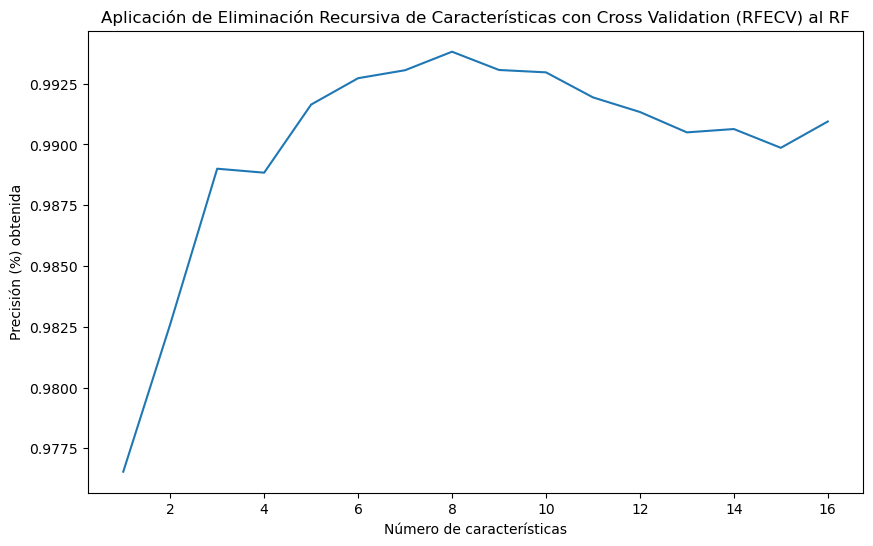
\includegraphics[width=0.85\textwidth]{img/desarrollo/rf/rfecv.png}
  \caption{Análisis de la precisión del modelo en función del número de características empleadas}
  \label{fig:rfecv}
\end{figure}

Por consiguiente, se entra en el funcionamiento de la segunda técnica a emplear, denominada como selección invariante de características (del inglés \textit{Univariate feature selection}) \cite{kbest}. 


% # In this method we need to choose how many features we will use. For example, will k (number of features) be 5 or 10 or 15? 
% # The answer is only trying or intuitively. I do not try all combinations but I only choose k = 5 and find best 5 features.

% #In univariate feature selection, we will use SelectKBest that removes all but the k highest scoring features.



%Univariate feature selection works by selecting the best features based on univariate statistical tests. It can be seen as a preprocessing step to an estimator. Scikit-learn exposes feature selection routines as objects that implement the transform method:

% SelectKBest removes all but the 
% highest scoring features

% SelectPercentile removes all but a user-specified highest scoring percentage of features

% using common univariate statistical tests for each feature: false positive rate SelectFpr, false discovery rate SelectFdr, or family wise error SelectFwe.

% GenericUnivariateSelect allows to perform univariate feature selection with a configurable strategy. This allows to select the best univariate selection strategy with hyper-parameter search estimator.
%These objects take as input a scoring function that returns univariate scores and p-values (or only scores for SelectKBest and SelectPercentile):For regression: r_regression, f_regression, mutual_info_regressionFor classification: chi2, f_classif, mutual_info_classif The methods based on F-test estimate the degree of linear dependency between two random variables. On the other hand, mutual information methods can capture any kind of statistical dependency, but being nonparametric, they require more samples for accurate estimation. Note that the -test should only be applied to non-negative features, such as frequencies.






\subsubsection{Ejecución y validación de los modelos}
\label{sec:rf4}

% Please find below these metrics formulas (TP = # True Positives, TN = # True Negatives, FP = # False Positives, FN = # False Negatives):

% Accuracy = (TP + TN) / (TP + TN + FP + FN)

% Precision = TP / (TP + FP)

% Recall = TP / (TP + FN)

% F1 Score = 2 * Precision * Recall / (Precision + Recall)



%Los pliegues, también conocidos como "folds" en inglés, se refieren a las divisiones que se hacen en el conjunto de datos durante la validación cruzada. La validación cruzada es una técnica utilizada para evaluar el rendimiento de un modelo de aprendizaje automático. Divide el conjunto de datos en múltiples subconjuntos llamados pliegues y utiliza estos pliegues de manera rotativa para entrenar y evaluar el modelo.



%%%%%%%


%calcular correlacion
%https://www.kaggle.com/code/saharnazhaji/solar-power-ml


%https://www.analyticsvidhya.com/blog/2021/10/an-introduction-to-random-forest-algorithm-for-beginners/
%se podria indicar aqui que criterio y que modelo (bara,wax) da mas problemas


%dibujar topo link con errores





